% Passover Seder Liturgy
\documentclass[10pt,oneside,footinclude=true,headinclude=true]{scrbook} % KOMA-Script book
\usepackage[LHE,T1]{fontenc}
\usepackage{lipsum}
\usepackage[linedheaders,manychapters,parts]{classicthesis} % ,manychapters
%\usepackage[osf]{libertine}
\usepackage[paperheight=8.5in,paperwidth=5.5in,margin=0.8in]{geometry}
\usepackage{graphicx}
\usepackage[english]{babel}

\usepackage{paracol}
\usepackage{transparent}

%\usepackage{palatino}

% Helper functions.
\newcommand\recitwidth{7.7cm}
\newcommand\oldrecite[2]{ \ifthenelse{\equal{#1}{All}} {\textbf{#1} : & \textbf{\small #2}} {#1 : & \small #2} }
\newcommand\recitecol[2]{
	\small{
		\begin{paracol}{2}
		\columnratio{0.15,0.85}
			\begin{leftcolumn}
			#1 :
			\end{leftcolumn}
			\begin{rightcolumn}
			\noindent #2
			\end{rightcolumn}
		\end{paracol}
	}
}
\newcommand\recite[2]{
	\ifthenelse{\equal{#1}{All}}
	{\textbf{\recitecol{#1}{#2}}}
	{\recitecol{#1}{#2}}
}

\newcommand\quot[1]{
	\begin{quote}\textit{\small#1}\end{quote}
}

\newcommand\pagequot[1]{
	\newpage
	\clearscrheadfoot
	%\vspace*{\fill}
	\vspace*{\stretch{2}}
	\begin{center}
	\begin{minipage}[c]{8cm}
		#1
	\end{minipage}
	\end{center}
	%\vspace*{\fill}
	\vspace*{\stretch{3}}
}

\begin{document}

%---------------------------------------------------------------------------------------
%	TITLE PAGE
%---------------------------------------------------------------------------------------
\begin{titlepage}
\begin{center}
\large \hfill \vfill

\begingroup
\color{RoyalPurple}\spacedallcaps{The Jusman Family Passover Liturgy} \\ \bigskip % Title
\endgroup

\spacedlowsmallcaps{J.Jusman}
\vfill

\includegraphics[width=6cm]{TFZsuperellipse_bw} \\ \medskip % Picture

\textit{...And when I see the blood, I will pass over you...} \\ \medskip % Subtitle

April 2017\ -- version 1.2 % Time and version

\vfill
\end{center}
\end{titlepage}
    
\newpage
\clearscrheadfoot
\null

%---------------------------------------------------------------------------------------
%	TOC
%---------------------------------------------------------------------------------------
\tableofcontents 
\cleardoublepage % use \cleardoublepage here to avoid problems with pdfbookmark


%---------------------------------------------------------------------------------------
%	INTRODUCTION
%---------------------------------------------------------------------------------------
\pagequot{
\centering
\textit{
Let not the foreigner who has joined himself to the LORD
say, "The LORD will surely separate me from his people"...\\
\smallskip
...And the foreigners who join themselves to the LORD,\\
    to minister to him, to love the name of the LORD,\\
    and to be his servants,\\
everyone who keeps the Sabbath and does not profane it,\\
    and holds fast my covenant--\\
these I will bring to my holy mountain,\\
    and make them joyful in my house of prayer;\\
their burnt offerings and their sacrifices\\
    will be accepted on my altar;\\
for my house shall be called a house of prayer\\
    for all peoples.\\
}
\bigskip
\spacedlowsmallcaps{Isaiah 56:3, 6-7}
}

%---------------------------------------------------------------------------------------
\setcounter{chapter}{-1}
\chapter{Introduction}

Why?\\
\\
Why we Chinese/Indonesian people be doing these weird Jewish people things?\\
\\
A couple of reasons:
\begin{enumerate}
	\item{
		Because the Passover traditions are beautiful and they point to our savior Jesus ("Yeshua").
		\quot{Behold, the Lamb of God, who takes away the sin of the world! (John 1:29)}
	}
	\item{
		Because Yeshua himself celebrated Passover and followed a Jewish liturgy.
%		\quot{They are Israelites, and to them belong the adoption, the glory, the covenants, the giving of the law, the worship, and the promises. (Romans 9:4)}
		\quot{So Jesus sent Peter and John, saying, "Go and prepare the Passover for us, that we may eat it." (Luke 22:8)}
	}
	\item{
		Because what we call "communion" at church is actually a couple of elements from the Passover liturgy.
		\quot{For I received from the Lord what I also delivered to you, that the Lord Yeshua on the night when he was betrayed took bread, and when he had given thanks, he broke it, and said, "This is my body which is for you. Do this in remembrance of me." In the same way also he took the cup, after supper, saying, "This cup is the new covenant in my blood. Do this, as often as you drink it, in remembrance of me." (1 Corinthians 11:23-25)}
	}
	\item{
		Because the Exodus was experienced by non-Jewish people also.
		\quot{A mixed multitude also went up with them... (Exodus 12:38)}
	}
	\item{
		Because it is weird even to the Jewish people.
		\quot{And when you come to the land that the LORD will give you, as he has promised, you shall keep this service. And when your children say to you, "What do you mean by this service?" you shall say, "It is the sacrifice of the LORD's Passover, for he passed over the houses of the people of Israel in Egypt, when he struck the Egyptians but spared our houses." (Exodus 12:26-27)}
	}
	\item{
		Because the Passover is the first proper commandment of God to his people, even before the Ten Commandments.
		\quot{This day shall be for you a memorial day, and you shall keep it as a feast to the LORD; throughout your generations, as a statute forever, you shall keep it as a feast. (Exodus 12:14)}
	}
\end{enumerate}


\section{The Feast}
The Passover is the most commonly celebrated Jewish feast. The liturgy for the meal is called the "Seder," but the feast itself (and the holiday) is called "Pesach." It is the meal of Yeshua's "Last Supper" with his disciples.

\quot{And when the hour came, he reclined at table, and the apostles with him. And he said to them, "I have earnestly desired to eat this Pesach with you before I suffer. For I tell you I will not eat it until it is fulfilled in the kingdom of God." (Luke 22:14-15)}


\section{The Rhyme}

The Seder liturgy is summarized in a nice little rhyme that spells out the order of the whole meal. Each of these little words signifies a step in the order.\\
\\
Qaddesh Urchatz, Karpas Yachatz\\
Maggid Rachtza, Motzi Mattza\\
Maror Korekh, Shulchan Orekh\\
Tzafun Barekh, Hallel Nirtza


\section{The Liturgy}

The liturgy is based on 4 cups of blessing, which correspond to God's 4 promises to his people while they were still in Egypt, before they went through the Exodus. (There are 3 other promises that they didn't include, and I don't know why, but such is life) We are doing a simplified liturgy, instead of a full-fledged one. Many items have been removed from the traditional Seder for reasons of time and my own ignorance. Sorry =)\\
\\
Items needed for the liturgy:
\begin{enumerate}
	\item{Two candles}
	\item{Grape juice or wine}
	\item{Unleavened bread or Matzah}
	\item{A white cloth to wrap the unleavened bread}
	\item{A linen cloth/napkin to hide the Afikomen}
	\item{A water pitcher, a washing bowl or basin, a hand towel}
	\item{A green vegetable, e.g. celery or parsley: representing fertility and growth}
	\item{A bitter herb, e.g. horseradish: representing the bitterness of slavery}
	\item{A bowl of salt water or vinegar: representing sweat and tears during slavery, also representing the Red Sea}
	\item{An extra chair}
\end{enumerate}

\vspace{5mm}

\noindent Let's begin the liturgy.\\
\\
\small
Eldest Woman: Let the eldest woman in the house light up two candles. (Usually every Sabbath, the youngest female in the house lights up the candles. But for Pesach, it's the eldest woman.)\\

\columnratio{0.15,0.85}

%---------------------------------------------------------------------------------------
%	PART I
%---------------------------------------------------------------------------------------
\normalsize
\pagequot{
\centering
\textit{I am the LORD, and \textbf{I will bring you out} from under the burdens of the Egyptians, and \textbf{I will deliver you} from slavery to them, and \textbf{I will redeem you} with an outstretched arm and with great acts of judgment. \textbf{I will take you} to be my people,...}\\
\bigskip
\spacedlowsmallcaps{Exodus 6:6-8}
}

%---------------------------------------------------------------------------------------
\part{The First Cup: I Will Bring You Out}

\chapter{Qaddesh: Sanctify} 
\makebox[0pt][l]{%
%  \raisebox{-\totalheight}[0pt][0pt]{%
  \raisebox{-3in}[0pt][0pt]{%
    {\transparent{0.1}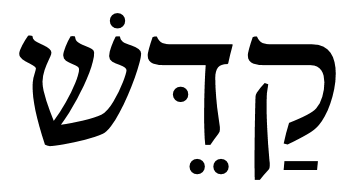
\includegraphics[width=3in]{qaddesh}}}}%
\normalsize
Step \thechapter: Sanctifying the wine.\\
\\
The Qiddush ("Sanctification") is a Sabbath blessing recited over wine or grape juice. It's recited weekly to sanctify the Sabbath, but also on Jewish holidays. The Shehecheyanu ("Who has given us life") is a blessing recited during special occasions, e.g. the beginning of a holiday or feast.

\vspace{5mm}
\hrule
\vspace{5mm}

The Qiddush:\\

\recite{Leader}{And there was evening and there was morning, the sixth day. Thus the heavens and the earth were finished, and all the host of them. And on the seventh day God finished his work that he had done, and he rested on the seventh day from all his work that he had done. So God blessed the seventh day and sanctified it, because on it God rested from all his work that he had done in creation.}

\recite{All}{Blessed are you O LORD our God, king of the universe, creator of the fruit of the vine.}

\recite{All}{[Pour a little wine for the person sitting to your left]}
\hfill

\recite{Leader}{Blessed are you O LORD our God, king of the universe, who sanctified us with his commandments, and was pleased with us, and invested us with his holy Sabbath in love and favor, as a memorial of the Creation. For it is foremost among the holy festivals commemorating the exodus from Egypt. For you chose us and sanctified us, out of all the peoples, and you invested us with your holy Sabbath in love and favor. Blessed are you O LORD, who sanctifies the Sabbath.}

\recite{All}{Amen.}

\vspace{5mm}
\hrule
\vspace{5mm}

\normalsize
The Shehecheyanu:\\

\recite{Leader}{Blessed are you O LORD our God, king of the universe, who has given us life and sustained us and brought us to this occasion.}

\recite{All}{Amen.}

\recite{All}{[Drink the first cup]}


%---------------------------------------------------------------------------------------
\chapter{Urchatz: And Wash}
\normalsize
Step \thechapter: Washing the hands.\\
\\
The youngest child in the house carries a towel around the table and dries everyone's hands.

\vspace{5mm}
\hrule
\vspace{5mm}

\recite{All}{[Pour water over the hands of the person to your right]}
\vspace{5mm}
\recite{Child}{[Dries hands with towel]}
\vspace{3mm}

\quot{Yeshua, knowing that the Father had given all things into his hands, and that he had come from God and was going back to God, rose from supper. He laid aside his outer garments, and taking a towel, tied it around his waist. Then he poured water into a basin and began to wash the disciples' feet and to wipe them with the towel that was wrapped around him.\\
\\
He came to Simon Peter, who said to him, "Lord, do you wash my feet?" Yeshua answered him, "What I am doing you do not understand now, but afterward you will understand." Peter said to him, "You shall never wash my feet." Yeshua answered him, "If I do not wash you, you have no share with me." Simon Peter said to him, "Lord, not my feet only but also my hands and my head!"\\
\\
Yeshua said to him, "The one who has bathed does not need to wash, except for his feet, but is completely clean. And you are clean, but not every one of you." For he knew who was to betray him; that was why he said, "Not all of you are clean." When he had washed their feet and put on his outer garments and resumed his place, he said to them, "Do you understand what I have done to you?.. (John 13:3-12)}


%---------------------------------------------------------------------------------------
\chapter{Karpas: Vegetable}
\normalsize
Step \thechapter: Eating vegetables dipped in the salt water.\\
\\
The green vegetable reminds us that it was springtime when the Exodus took place. It also represents growth and fertility of the Jewish people in Egypt. The salt water represents their sweat and tears during slavery, and also their crossing the Red Sea.\\
\\
\recite{All}{Blessed are you O LORD our God, king of the universe, creator of the fruit of the earth. Amen.}

\recite{All}{[Dip the vegetable in the salt water. Don't forget to shake off some salt water drops, resembling tear drops]}

\recite{All}{[Eat the vegetable]}


%---------------------------------------------------------------------------------------
\chapter{Yachatz: Divide}
\normalsize
Step \thechapter: Breaking the matzah.\\

\quot{Now as they were eating, Jesus took bread, and after blessing it broke it and gave it to the disciples, and said, "Take, eat; this is my body." (Matthew 26:26)}


%---------------------------------------------------------------------------------------
%	PART II
%---------------------------------------------------------------------------------------
\pagequot{
\centering
\textit{..., and I will be your God, and you shall know that I am the LORD your God, who has brought you out from under the burdens of the Egyptians. I will bring you into the land that I swore to give to Abraham, to Isaac, and to Jacob. I will give it to you for a possession. I am the LORD."}\\
\bigskip
\spacedlowsmallcaps{Exodus 6:6-8}
}

\part{The Second Cup: I Will Deliver You}


%---------------------------------------------------------------------------------------
\chapter{Maggid: Telling}
\normalsize
Step \thechapter: Telling the story.\\
\\
In this section we retell the story of the first Pesach and the Exodus of the Jewish people from Egypt. It begins with the youngest person asking the Four Questions, and then receiving Four Answers from the family. Everyone is encouraged to participate in the telling of the story. However, the actual telling of the story is usually done after the meal. I guess this makes sense, considering all the growling of stomachs and their ever-increasing demand for attention.\\
\\

\recite{Leader}{Let's get back to this section later after dinner and read Exodus 12.}

\recite{All}{[Pour a little wine for the person sitting to your right]}

\recite{All}{Blessed are you O LORD our God, king of the universe, creator of the fruit of the vine. Amen.}

\recite{All}{[Drink the second cup]}


%---------------------------------------------------------------------------------------
\chapter{Rachtza: Washing}
\normalsize
Step \thechapter: Washing the hands.\\
\\


%---------------------------------------------------------------------------------------
\chapter{Motzi Mattza: Bringing Out Matzah}
\normalsize
Step \thechapter: Eating the Matzah.\\

\recite{All}{Blessed are you O LORD our God, king of the universe, who brings forth bread from the earth. Amen.}

\recite{All}{[Eat the Matzah]}

The Passover Lamb has been sacrificed Corinthians.


%---------------------------------------------------------------------------------------
\chapter{Maror: Bitter Herb}
\normalsize
Step \thechapter: Eating the Bitter Herb.\\


%---------------------------------------------------------------------------------------
\chapter{Korekh: Sandwich}
\normalsize
Step \thechapter: Eating the Sandwich.\\


%---------------------------------------------------------------------------------------
\chapter{Shulchan Orekh: Preparing Table}
\normalsize
Step \thechapter: Eating the Meal.\\
\\
This is the eating part of the Feast, the actual Feasting itself.


%---------------------------------------------------------------------------------------
\chapter{Tzafun: Hidden}
\normalsize
Step \thechapter: Finding and uncovering and eating the afikomen.\\


\quot{Truly, you are a God who hides himself,\\
\hspace*{5mm}O God of Israel, the Savior.\\
All of them are put to shame and confounded;\\
\hspace*{5mm}the makers of idols go in confusion together.\\
But Israel is saved by the Lord\\
\hspace*{5mm}with everlasting salvation;\\
you shall not be put to shame or confounded\\
\hspace*{5mm}to all eternity.}


%---------------------------------------------------------------------------------------
%	PART III
%---------------------------------------------------------------------------------------
\pagequot{
\centering
\textit{...I began to weep loudly because no one was found worthy to open the scroll or to look into it. And one of the elders said to me, "Weep no more; behold, the Lion of the tribe of Judah, the Root of David, has conquered, so that he can open the scroll and its seven seals." And between the throne and the four living creatures and among the elders I saw a Lamb standing, as though it had been slain...\\
\vspace{2mm}
...And they sang a new song, saying,\\
"Worthy are you to take the scroll\\
\hspace*{5mm}and to open its seals,\\
for you were slain, and by your blood you ransomed people for God\\
\hspace*{5mm}from every tribe and language and people and nation,\\
and you have made them a kingdom and priests to our God,\\
\hspace*{5mm}and they shall reign on the earth."}\\
\bigskip
\spacedlowsmallcaps{Revelation 5:4-6, 9-10}
}

\part{The Third Cup: I Will Redeem You}


%---------------------------------------------------------------------------------------
\chapter{Barech: Bless}
\normalsize
Step \thechapter: Blessing after the meal.\\

\recite{Leader}{Blessed are you O LORD our God, king of the universe, who nourishes the whole world with goodness, with grace, kindness, and compassion. He gives bread to all flesh, for his love endures forever. And through his great goodness we have never lacked, nor will we lack food forever, for the sake of his great name. For he is God, who nourishes and sustains all, and does good to all, and prepares food for all his creatures which he created. Blessed are you O LORD, who nourishes all.}

\recite{All}{Amen.}

\recite{All}{[Pour a little wine for the person sitting to your right]}

\recite{All}{Blessed are you O LORD our God, king of the universe, creator of the fruit of the vine. Amen.}

\recite{All}{[Drink the third cup]}


%---------------------------------------------------------------------------------------
%	PART IV
%---------------------------------------------------------------------------------------
\normalsize
\pagequot{
\centering
\textit{Then she fell on her face, bowing to the ground, and said to him, "Why have I found favor in your eyes, that you should take notice of me, since I am a foreigner?"}\\
\bigskip
\spacedlowsmallcaps{Ruth 2:1O}
}

\part{The Fourth Cup: I Will Take You}


%---------------------------------------------------------------------------------------
\chapter{Hallel: Praise}
\normalsize
Step \thechapter: Song of praise.\\

\footnotesize
\columnratio{0.4,0.6}
\begin{paracol}{2}
\begin{leftcolumn}
\noindent Ilu hotzi, hotzi'anu\\
Hotzi'anu miMitzrayim\\
Hotzi'anu miMitzrayim\\
Dayenu\\
\\
Day, day yenu (3x)\\
Dayenu\\
Dayenu!\\
\\
Ilu natan, natan lanu\\
Natan lanu et haTorah\\
Natan lanu et haTorah\\
Dayenu\\
\\
Day, day yenu...\\
\\
Ilu shalach, shalach lanu\\
Shalach lanu et Mashiach\\
Shalach lanu et Mashiach\\
Dayenu\\
\\
Day, day yenu...\\
\end{leftcolumn}
\begin{rightcolumn}
\noindent Had he only brought us, brought us out\\
Brought us out from Egypt\\
Brought us out from Egypt\\
Then it would have been enough\\
\\
It would have been enough (3x)\\
It would have been enough\\
It would have been enough!\\
\\
Had he given, given to us\\
Given to us the Torah\\
Given to us the Torah\\
Then it would have been enough\\
\\
It would have been enough...\\
\\
Had he sent, sent to us\\
Sent to us the Messiah\\
Sent to us the Messiah\\
Then it would have been enough\\
\\
It would have been enough...\\
\end{rightcolumn}
\end{paracol}

\columnratio{0.15,0.85}

\tiny
\recite{All}{[Pour a little wine for the person sitting to your right]}

\recite{All}{Blessed are you O LORD our God, king of the universe, creator of the fruit of the vine. Amen.}

\recite{All}{[Drink the fourth cup]}

\quot{And when they had sung a hymn, they went out to the Mount of Olives. Matt 26:30, Mark 14:26}


%---------------------------------------------------------------------------------------
\normalsize
\pagequot{
\centering
\textit{And Abraham took the wood of the burnt offering and laid it on Isaac his son. And he took in his hand the fire and the knife. So they went both of them together. And Isaac said to his father Abraham, "My father!" And he said, "Here I am, my son." He said, "Behold, the fire and the wood, but where is the lamb for a burnt offering?" Abraham said, "God will provide for himself the lamb for a burnt offering, my son." So they went both of them together.}\\
\bigskip
\spacedlowsmallcaps{Genesis 22:6-8}
}



%---------------------------------------------------------------------------------------
\chapter{Nirtza: Pleasing}
\normalsize
Step \thechapter: Prayer that our service be pleasing and acceptable to God.\\



\quot{Speak tenderly to Jerusalem,\\
\hspace*{5mm}and cry to her\\
that her warfare is ended,\\
\hspace*{5mm}that her iniquity is pardoned (nirtza),\\
that she has received from the LORD's hand\\
\hspace*{5mm}double for all her sins. (Isaiah 40:2)}


%---------------------------------------------------------------------------------------
%	APPENDIX
%---------------------------------------------------------------------------------------

\appendix
\cleardoublepage
\part{Appendix}


%---------------------------------------------------------------------------------------
\chapter{The Door}
<Exodus 12:7>
\quot{Then they shall take some of the blood and put it on the two doorposts and the lintel of the houses in which they eat it.}

\noindent...the blood...

\quot{So Jesus again said to them, "Truly, truly, I say to you, I am the door of the sheep."}

\noindent...the door...\\
...the way...

\quot{"I am the way, and the truth, and the life."}

\noindent...the life...

\quot{For the life of every creature is its blood: its blood is its life. Therefore I have said to the people of Israel, You shall not eat the blood of any creature, for the life of every creature is its blood. Whoever eats it shall be cut off.}

\quot{For the life of the flesh is in the blood, and I have given it for you on the altar to make atonement for your souls, for it is the blood that makes atonement by the life.}

\noindent...the life...is in the blood...\\
...without the blood, there is no life...\\
...without the blood, there is no atonement...\\
...without the blood, the door is just the door, it is not the way...\\
...but with the blood, the door becomes the way, the gate...\\

\noindent...the way...the way to where?

\quot{Jesus said to him, "I am the way, and the truth, and the life. No one comes to the Father except through me."}

\noindent...the way to the Father...

\quot{Then you shall say to Pharaoh, 'Thus says the LORD, Israel is my firstborn son,  and I say to you, "Let my son go that he may serve me."'}

\noindent...that the son...may go to the Father...\\
...that the sheep...may go find pasture...

\quot{Know that the LORD, he is God!\\
\hspace*{5mm}It is he who made us, and we are his;\\
\hspace*{5mm}we are his people, and the sheep of his pasture.}

\quot{For he is our God,\\
\hspace*{5mm}and we are the people of his pasture,\\
\hspace*{5mm}and the sheep of his hand.}

\quot{Today, if you hear his voice,...}

\quot{I will surely assemble all of you, O Jacob;\\
\hspace*{5mm}I will gather the remnant of Israel;\\
I will set them together\\
\hspace*{5mm}like sheep in a fold,\\
like a flock in its pasture,\\
\hspace*{5mm}a noisy multitude of men.}

\quot{He who opens the breach goes up before them;\\
\hspace*{5mm}they break through and pass the gate,\\
\hspace*{5mm}going out by it.\\
Their king passes on before them,\\
\hspace*{5mm}the LORD at their head.}

\quot{"To him the gatekeeper opens. The sheep hear his voice, and he calls his own sheep by name and leads them out."}

\quot{Moses spoke to the LORD, saying, "Let the Lord, the God of the spirits of all flesh, appoint a man over the congregation who shall go out before them and come in before them, who shall lead them out and bring them in, that the congregation of the LORD may not be as sheep that have no shepherd."\\
\\
So the LORD said to Moses, "Take Joshua the son of Nun, a man in whom is the Spirit, and lay your hand on him.\\
\\
And he shall stand before Eleazar the priest, who shall inquire for him by the judgment of the Urim before the Lord. At his word they shall go out, and at his word they shall come in, both he and all the people of Israel with him, the whole congregation."}

\quot{"I am the door. If anyone enters by me, he will be saved and will go in and out and find pasture."}

\quot{Only be sure that you do not eat the blood, for the blood is the life, and you shall not eat the life with the flesh. Deut 12:23}

\quot{So Jesus said to them, "Truly, truly, I say to you, unless you eat the flesh of the Son of Man and drink his blood, you have no life in you." John 6:53}

\quot{And the Word became flesh and dwelt among us...}

\quot{"Man shall not live by bread alone,\\
\hspace*{5mm}but by every word that comes from the mouth of God."}

\quot{"I am the living bread that came down from heaven. If anyone eats of this bread, he will live forever. And the bread that I will give for the life of the world is my flesh."}

\quot{They shall eat the flesh that night, roasted on the fire; with unleavened bread and bitter herbs they shall eat it.}
<Exodus 12:8>


%---------------------------------------------------------------------------------------
\chapter{One and The Same}
by Kyle Matthews and Pete Carlson

How can you explain\\
He that is the Root of David, yet at the same time is the Branch?\\
The Shepherd, yet at the same time the Lamb?\\
The Lord, yet the Slave?\\
The Healer, yet the Wounded One?\\
Son of God the Creator, yet Son of Man the Creature?\\
The First and the Last? The Beginning and the End?\\
\\
So high and mighty, yet closer than a friend?\\
The holy God of Heaven and the humble man who bore\\
Who bore my shame are one, one and the same\\

\end{document}
